\documentclass{article}
\usepackage{cite}
\usepackage{graphicx}
\usepackage{listings}
\usepackage[pdf]{pstricks}

\usepackage{color}
\definecolor{gray}{rgb}{0.4,0.4,0.4}
\definecolor{darkblue}{rgb}{0.0,0.0,0.6}
\definecolor{cyan}{rgb}{0.0,0.6,0.6}
\definecolor{red}{rgb}{0.8,0.0,0.2}
\definecolor{pink}{rgb}{0.8, 0.2, 0.8}
\definecolor{green}{rgb}{0.0, 0.8, 0.2}

\lstset{
  basicstyle=\ttfamily,
  columns=fullflexible,
  showstringspaces=false,
  commentstyle=\color{gray}\upshape
}

\lstdefinelanguage{XML}
{
  morestring=[b]",
  %morestring=[s]{>}{<},
  morecomment=[s]{<?}{?>},
  morecomment=[s]{<!--}{-->},
  stringstyle=\color{red},
  identifierstyle=\color{darkblue},
  keywordstyle=\color{pink},
  commentstyle=\color{green},
  morekeywords={xmlns,version,type, ToM, name, operator, value, probability}% list your attributes here
}


\begin{document}

\title{Extending Believable Agent Frameworks with Predicate
  Logic Dialogue Generation}
\author{Kaylen Wheeler}

\maketitle

\begin{abstract}

Despite advances in graphics, physics, and AI, modern video games are
still lacking in believable social simulation.  Story, dialogue, and
character behaviour are more often scripted than allowed to emerge
dynamically.  The more complex and interactive stories in modern games
may allow the player to experience different paths in dialogue trees,
but such trees are still required to be manually created by authors.
Recently, there has been research on methods of creating emergent
believable behaviour \cite{Acton2009,Mascarenhas,Mateasc}, but these are
lacking true dialogue construction.  Because the mapping of natural
language sentences to meaningful computational representations
(logical forms) is still an unsolved problem \cite{Zettlemoyer2004}, it
may be best to represent inter-character dialogue as logical forms.
The proposed thesis will extend an existing believable agent
framework with a predicate logic-based dialogue module that will
allow for true construction and interpretation of dialogue by
non-player characters.

\end{abstract}

\section{Introduction}

Throughout the history of video gaming, the majority of efforts to
increase believability have focused on advancement in graphics and
physics, powered largely by advances in computer hardware.  Modern
games often have near-photorealistic graphics and highly believable
physical simulation.  However, advances in AI, although present, have
not added much to believabilty.  Rather, developments in game AI are
focused on providing challenging and interesting gameplay by creating
agents that can either cooperate or compete with the player.  Such
agents, although effective in creating entertaining gameplay, fail to
create believable characters, specifically with regards to social
behaviour.

In addition to social behaviour, the ability to generate dialogue
dynamically is also lacking.  Modern games which are praised for their
complex dialogue systems, such as the \emph{Mass Effect} series \cite{BioWare2007}
 do not in fact have their characters generate dialogue, but
rather select from pre-written (and voiced) dialogue based on certain
conditions.  Even experiments in interactive drama such as Facade
\cite{Mateasc} rely on complex ways of selecting from a set of existing
dialogue acts.  Facade is a highly variable game experience taking
only about 20 minutes to play through and consisting of a very limited
environment (a single room with one player character and two NPC's), and
yet several hundred thousand lines of code were written of handle all
possible dialogue acts\cite{Mateas}.  Clearly, such an approach is not
scalable to open world, multi-agent environments.

Believable agent frameworks are already in place which simulate
emotional and social interactions.  These systems allow for autonomous
agents to form goals based on their current emotional state and social
relations, and perform actions to satisfy those goals.

The proposed thesis will involve the implementation of an extension dialogue module
to FAtiMA\cite{Mascarenhas}, an existing believable agent framework.
Currently, the agents in FAtiMA are limited to selecting from an
existing finite set of actions to perform based on their goals and
current state.  Using the same goals and current state, the new dialogue
module would allow agents to perform not only action selection, but
action construction, creating arbitrary logical expressions to
communicate with other agents.  Additionally, the module will allow for
the interpretation of such logical expressions to affect the current
state of an agent.

\section{Background and Previous Work}

This thesis will involve the synthesis of both Believable Agent
Frameworks (abbreviated here as BAF) and Natural Language Processing
(NLP).  This section will provide background and previous research
from each of these areas.

\subsection{Believable Agent Frameworks}

A BAF is any framework that simulates the social and emotional
behaviours of humans in a believable way.  The term ``Believable'' is
difficult to define because it is subjective by nature.  However, it
is often suggested that believability is not truly an attempt to fool
the user into actually believing what is presented; it is rather an
attempt to allow the user to willingly suspend disbelief. \cite{Acton2009}

A well-known attempt to create more believable narrative and gameplay
is the Facade
project\cite{Mateas}.  Facade is a one-act interactive drama with a
natural written language interface.  The player takes on the role of a
character visiting a married couple, and is able to converse in
real-time with the other two characters by typing natural language
text.

Although Facade was created to select appropriate responses to many
situations, each of these responses was hand-authored.  Additionally,
natural language input from the user was not intrepreted to its
fullest possible extent by the program.  Rather, surface text
processing was used which searched user input for a number of key
words and phrases and mapped it to one of a finite, pre-defined set of
discourse acts. \cite{Mateasa}  In some ways, Facade can be considered
similar to dialogue trees in games such as \emph{Mass Effect}, but with an
interface that gives the illusion of natural language interaction.

Some of the creators of Facade were also involved in the
creation of the ``Comme il Faut''(CiF)\cite{Mccoy2010}, a social AI
system.  The intention of CiF was to provide a ``system for authoring playable social
models''\cite{Mccoy2010}.  Rather than authoring dialogue trees, which
the authors called ``burdensome''  and ``highly constrained'', the
Social AI System  would allow the authoring of a ``space of possible
stories''.  Through the definition of social and cultural rules that
can be applied to a given social state, believable social behaviour is
allowed to emerge.

CiF was used to implement the game \emph{Prom Week} [TODO: Cite the
  game itsetf?].  \emph{Prom Week} pioneered what the creators termed ``Social
Physics''\cite{Mccoy2011} -- intuitive rules of social
interaction that could guide the user's gameplay toward accomplishing
the game's goals, similar to how physics are used in many puzzle
games.  However, like Facade, and despite its advanced modelling of
social and emotional phenomena, the dialogue is still composed of a
finite number of templates that are selected in the appropriate
situations.

A more easily accessible (in terms of source code) and more modular
BAF is the FearNot Affective Mind Architecture (FAtiMA)
\cite{Mascarenhas}.  FAtiMA was developed initially as an engine for
\emph{FearNot!}[TODO: Cite fearnot game?], a serious game aimed at
teaching school children between ages 8 and 12 how to deal with being
bullied.

FAtiMA has a number of modules, each based around modelling aspects of
believable agents.  These include modules for modelling Theory of
Mind\cite{Marsella}, memory, emotional intelligence, dialogue, and
others.  It also has the ability to be easily extended by adding new
modules.  This feature allows different models of the same phenomena
to be implemented and tested for validity within the same framework
(e.g. evaluating different theories of emotion appraisal for their
believability).

In terms of dialogue, FAtiMA currently has a module that maps Theory
of Mind (ToM) - related goals to pre-defined discourse actions.  Theory of
Mind goals differ from other goals in that they seek to affect the
state of another agent's beliefs rather than the state of the world
itself.  These dialogue acts, however, are not creted dynamically and
must be manually authored and explicitly mapped to corresponding agent
goals.


\subsection{Natural Language Processing}

Natural language processing is still an ongoing area of research.  Recent
developments have lead to more advanced search engines and data mining 
techniques, as well as computer-aided natural language translation.  However,
the problem of mapping natural language sentences to meaningful forms that can
be effectively interpreted by a computer is still a very open problem.

Zettlemoyer \cite{Zettlemoyer2004} has conducted some interesting research
on the topic of mapping natural language sentences to lambda calculus
expressions, which can be easily represented as sentences in
first-order logic.  His research makes use of combinatory categorical
grammars (CCG) \cite{Steedman2003} generated by advanced machine
learning techniques in order to parse sentences of various natural
languages.

An example of a mapping of natural language to lambda calculus is
demonstrated below.  Here, the sentence ``What states border Texas?''
is mapped to an equivalent lambda expression.  The expression takes as
a parameter a single unbound variable \emph{x}, which must satisfy the
condition of being a state and bordering texas.  When the expression
is used as a query to a knowledge base, \emph{x} unifies with all
values that satisfy both conditions.

\begin{figure}[h!]
\begin{center}
{
\center ``What states border Texas?''}

\[
 \lambda x.(state(x) \wedge  border(x,Texas))
\]
\[
 x = \{NewMexico, Oklahoma, Arkansas, Louisiana\}
\]

\end{center}
\end{figure}

Although the specifics of the theory and implementation are beyond the
scope of -- and likely of little relevance to -- this proposal, the
important realization is that natural language sentences can be
transformed into these forms, as well as the fact that software exists
that can accomplish this transformation[TODO: Reference Openccg?].
Using software to translate logical expressions into natural language
could allow the creation of language-independent dynamic dialogue
systems that can be easily localized into different languages.


\section{Problem Description and Proposed Solution}

Although many of the Believable Agent Frameworks researched so far
have had extensive flexibility in the use of authored dialogue, the
fact still remains that the dialogue must be authored.  For each
dialogue act, its representation (i.e. words used in the dialogue) as well as
each of its effects on the world or other agents must be explicitly
defined.  Additionally, explicit mappings between agents' states or
goals to dialogue actions must be provided (e.g. the goal to make
another character laugh must explicitly relate to the ``tell joke''
action).

The proposed solution is to create a system that alleviates the need
to explicitly author dialogue acts.  Rather than providing a set of
mappings between domain-specific dialogue acts and goals, a
domain-independent module will be created that constructs dialogue
acts to match goals.  The system will be implemented as an extension
to FAtiMA's existing dialogue system.

FAtiMA uses knowledge bases to represent both the state of the world
and the beliefs of individual agents.  These knowledge bases have
capabilities similar to first-order logic systems.  Rather than
generating natural language dialogue, first-order logic expressions
will be created to accomplish the goals that have been specified by
the agents.

If possible, the solution may also include natural language
``rendering'' and ``de-rendering'' modules.  These would allow logical
expressions to be converted to and from natural language sentences.
This is not necessary in the implementation, but may be included if
time allows in order to demonstrate how natural language could further
improve believability.

\subsection{Illustrative Example}

To understand the differences between authoring and generating
dialogue actions, an example will be provided.  This represents a
hypothetical scenario involving two characters -- Good Guy and Bad
Guy, who complement and insult one another.  Three main components are
defined for each character -- goals, action tendenceies, and
actions.  These defined in pseudocode, visible in figure
~\ref{example_goals}.

\begin{figure}[h!]
  
  \begin{center}
    \large{Good Guy}
  \end{center}
  
  Goals:
  \[
  isHappy(target)
  \]

  Action Tendencies:
  \[
  \lambda x.\lambda p.(knows(self, mother(x,self) \wedge good(p) \wedge p(x)) \mapsto isHappy(self))
  \]
  \[
  \lambda x.\lambda p.(knows(self, mother(x,self) \wedge \neg bad(p) \wedge p(x)) \mapsto \neg isHappy(self))
  \]

  Actions:
  \[
  complement(target) \mapsto knows(target, isHandsome(target))
  \]

  \[\]

  \begin{center}
    \large{Bad Guy}
  \end{center}
  
  Goals:
  \[
  \neg isHappy(target)
  \]

  Action Tendencies:
  \[
  \lambda p.(knows(self, good(p) \wedge p(self)) \mapsto isHappy(self))
  \]

  Actions:
  \[
  \lambda x.(insultMother(target) \mapsto knows(target, mother(x, target) \wedge
  isFat(x))) 
  \]
  
  \[\]

  \begin{center} \large{General Knowledge} \end{center}

  \[
  good(isHandsome)
  \]
  \[
  good(isThin)
  \]
  \[
  bad(isUgly)
  \]
  \[
  bad(isFat)
  \]

  \caption{An example of goal, action tendency, and action
    specification for two agents.  The left side of the $\mapsto$ symbol
    represents the preconditions in the case of action tendencies and
    action definitions in the case of actions.  The right side
    represents the effect.  The variables \emph{self} and
    \emph{target} are references to the agent's self and another in
    the environment.  Unbound variables are introduced with $\lambda$-notation.}
  \label{example_goals}

\end{figure}

Goals represent states that the agents are striving to achieve.  In
the case of Good Guy, his goal is that \emph{target}(i.e. Bad Guy)
should be happy.  Bad Guy's goal, on the other hand, is that
\emph{target}(i.e. Good Guy) should not be happy.

Action tendencies represent how agents act when faced with certain
situations.  The particular situations illustrated here involve
knowledge, and are defined with the \emph{knows} predicate.  (At the
moment, FAtiMA supports action tendencies in response to events.  To
support this dialogue system, it will need to be extended to analyze
changes in knowledge bases.)  For Good Guy's action tendencies, an
unbound variables \emph{x} and \emph{p} are introduced.
The variable \emph{x} unifies with \emph{self}'s mother, while \emph{p}
unifies with some predicate, which is \emph{good} or \emph{bad}.
The results (after the $\mapsto$ symbol) are either happiness or uhnappiness.  Thus, the
action tendencies for Good Guy can be described as ``If I know something
good about my mother, I am happy.'' and ``If I know something bad about my mother, I
am not happy.''.  Similarly, Bad Guy's action tendency is ``If I know
something good about me, I am happy.''.

A finite set of actions is defined, representing potential effects
that agents may have on the world.  A continuous partial-order planner
\cite{Paiva2005, Russell2003} is used to construct plans composed of
sequences of actions that achieve the agent's goals.  However, the
actions in the sequence may only be selected from a finite,
pre-defined set of actions.  The goal of this thesis will be to allow
for actions to be constructed from the goal they are trying to achieve.

\subsubsection{Example Plans}

Two examples are shown in figures ~\ref{plan_selection} and ~\ref{plan_construction}.
The first example shows an example of how an agent's plan would be
constructed if using action selection (the current method), while the
second shows how a plan might be created using action construction
(the proposed method.  In the example scenario, Bad Guy is attempting
to fulfill the goal of making some target (Good Guy) feel unhappy.

For each figure, the first few steps are the same.  We'll start with
figure ~\ref{plan_selection}.  First, the goal of causing
unhappiness is identified.  Using knowledge about the Good Guy's
action tendencies, Bad Guy is able to discern that Good Guy would
feel unhappy if he knew something bad about his mother.  Bad Guy's existing
set of actions are then analyzed to determine if any of them can
cause Good Guy to know something bad about his mother.  Because the
predicate \emph{isFat} is idenified in the general knowledge base as
being \emph{bad}, the action \emph{insultMother} is chosen to satisfy the
goal.

The important difference in ~\ref{plan_construction} is that Bad Guy's
set of actions are not analyzed for a solution.  Instead, an action
is constructed.  Bad Guy is able to construct logical statements
that will change Good Guy's knowledge state.  In this case, the posisble
statements involve bad things said about Good Guy's mother.  Using
an expression-construction algorithm (which is yet to be determined),
Bad Guy is able to construct a variety of expressions which have the
desired effect.  In this case, the expressions constructed equate to
``Your mother is fat.'' and ``Your mother is ugly.''.  In the current
system, the fat and ugly insults would have had to be separately
authored.  The proposed system will enable dynamic and varied
dialogue construction for any knowledge-related goals.

\begin{figure}[h!]
  
  \begin{center}\large{Action Selection}\end{center}

  Goal:
  $$
  \neg isHappy(target)
  $$

  Knowledge about target:
  \[
  \lambda x.\lambda p.(knows(target, mother(x,target) \wedge good(p) \wedge p(x)) \mapsto isHappy(target))
  \]
  \[
  \lambda x.\lambda p.(knows(target, mother(x,target) \wedge bad(p) \wedge p(x)) \mapsto \neg isHappy(target))
  \]

  Planner infers that the effect:
  \[
  \neg isHappy(target)
  \]

  Can be accomplished with:
  \[
  \lambda x.\lambda p.(knows(self, mother(x,target) \wedge bad(p) \wedge p(x)) \mapsto \neg isHappy(target))
  \]

  This becomes the new Goal.

  The planner analyzes the available actions:
  \[
  \lambda x.(insultMother(target) \mapsto knows(target, mother(x, target) \wedge
  isFat(x))) 
  \]

  If \emph{p} unifies with \emph{isFat}, it satisfies $bad(p)$.  The planner infers that
  the action \emph{insultMother} will have an effect identical to the goal it wants to accomplish.
  Therefore, Bad Guy's plan is to take the action:
  
  \[
  insultMother(target)
  \]

  \caption{Bad Guy's plan for insulting Good Guy's mother with action selection.}
  \label{plan_selection}
\end{figure}

\begin{figure}[h!]
  
  \begin{center}\large{Action Construction}\end{center}

  Goal:
  $$
  \neg isHappy(target)
  $$

  Knowledge about target:
  \[
  \lambda x.\lambda p.(knows(target, mother(x,target) \wedge good(p) \wedge p(x)) \mapsto isHappy(target))
  \]
  \[
  \lambda x.\lambda p.(knows(target, mother(x,target) \wedge bad(p) \wedge p(x)) \mapsto \neg isHappy(target))
  \]

  Planner infers that the effect:
  \[
  \neg isHappy(target)
  \]

  Can be accomplished with:
  \[
  \lambda x.\lambda p.(knows(target, mother(x,target) \wedge bad(p) \wedge p(x)) \mapsto \neg isHappy(target))
  \]

  This becomes the new Goal.

  There are no actions for the planner to select from.  Instead it generates speech
  actions.

  \[
  talkAction_1(me, you) \mapsto communicate(me, you, \lambda x.(mother(x, you) \wedge isFat(x)))
  \]
  \[
  talkAction_2(me, you) \mapsto communicate(me, you, \lambda x.(mother(x, you) \wedge isUgly(x)))
  \]

  Because \emph{p} can unify with anything that is \emph{bad}, it can either unify with
  \emph{isUgly} or \emph{isFat}, allowing new and interesting insults to be generated
  without the need for explicit authoring.

  Bad Guy therefore has two possible plans of action:

  \[
  talkAction_1(self, target)
  \]
  \[
  talkAction_2(self, target)
  \]

  \caption{Bad Guy's plan for insulting Good Guy's mother with action construction.}
  \label{plan_construction}
\end{figure}

\section{Design}

\subsection{Overview of FAtiMA}

FAtiMA is an Agent architecture with planning capabilities designed to use emotions
and personality to influence the agent's behaviour\cite{Mascarenhas}.  FAtiMA consists
of a core system (FAtiMA.Core) that allows external modules to be used to implement more
complex behaviour.  However, this section will focus on the core components.

In order to better understand descriptions of the system, the core concepts and 
terminology will be introduced here.

\begin{description}

\item[Agent]
  Agents are the primary actors in FAtiMA.  They represent entities which have emotions
  and goals, and may take action to affect their surroundings and other agents.

\item[World]
  In order for FAtiMA agents to function, they must exist in a world.  A world contains
  a set of objects and other agents that exist together and can affect one another.

\item[Scenario]
  A scenario consists of information that is necessary to describe the world.  In
  FAtiMA, scenarios are specified in XML files listing the agents and objects
  in the world.

\item[Appraisal]
  The process of determining how an agent should process an event, and how that event should
  affect their emotional state.
  
\item[Coping]
  The process of selecting, based on the agent's current emotional state, which actions to
  take.

\item[Reactive Level]
  For both appraisal and coping, this level determines instinctive reactions that are
  executed immediately (e.g. flinching when getting hit).  These correspond to an
  agent's \emph{action tendencies}, and represent reactions that the agent has
  no control over.

\item[Deliberative Level]
  This level enables the agents to construct long-term complex plans for achieving
  their goals.

\item[Memory]
  FAtiMA supports both episodic and semantic memory.  Episodic memory represents 
  short-term memory relating to events that have taken place, while semantic
  memory is represented as a knowledge base.

\item[Knowledge Base (KB)]
  Knowledge bases are the primary means of long-term information storage for
  an agent.  A KB represents the agent's perceived state of the world.  Information
  is represented through use of predicates representing facts or relations
  between objects in the world.  The predicates used here are similar to those
  used in logic programming systems such as Prolog.

\item[Goal]
  Goals represent states of the world or of a knowledge base that agents want
  to achieve.  In order to achieve goals, plans are created from actions.

\item[Action]
  An action represents a single effect that the agent may perform on the world.
  Each action will affect a change on the state of the world or a knowledge base.
  Currently, actions are pre-defined, but the aim here is to enable construction
  of those actions which transmit information (i.e. affect a knowledge base).

\item[Plan]
  Plans bring all the previously mentioned components together and make them
  work.  Through planning, agents can determine which sequences of actions (if any)
  can be used to accomplish their goals.

\item[Sensors]
  Refers to the means by which agents detect events in the world.  At the moment,
  these are triggered by actions taken by other agents or objects.  For the 
  purpose of the new system, they will have to monitor changes to knowledge bases.

\item[Effectors]
  Processes through which the agent can affect the world (i.e. actions).

\end{description}

\begin{figure}[h]
  \resizebox{1.0\textwidth}{!}{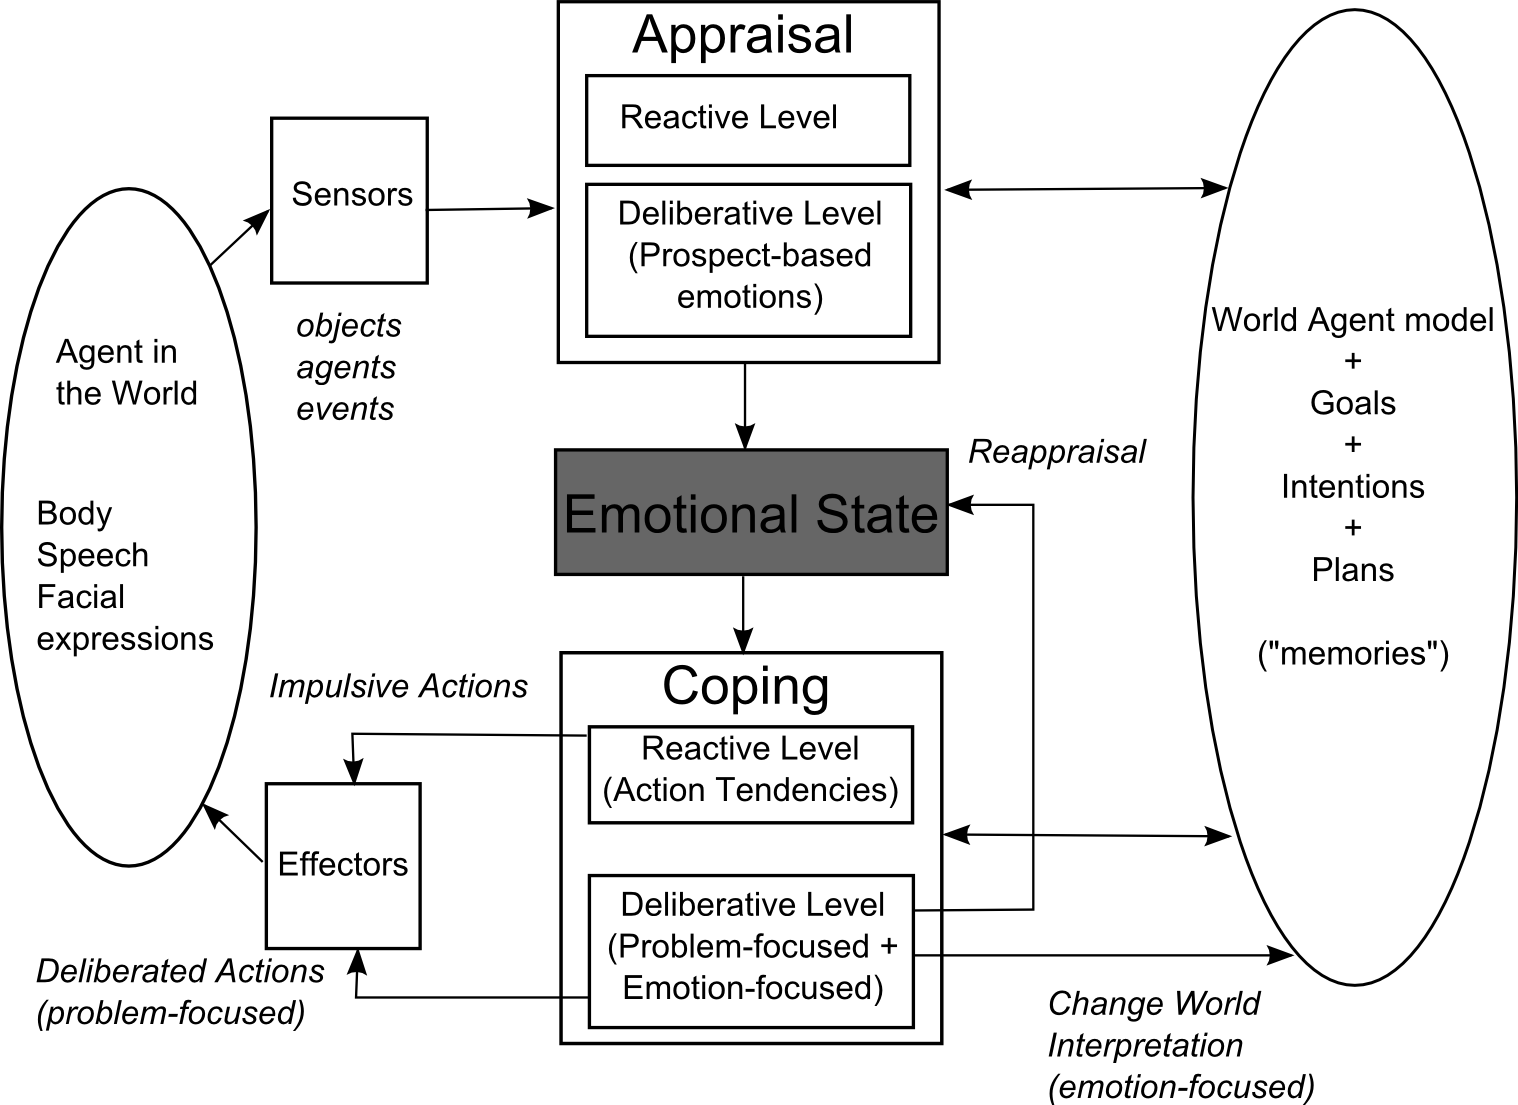
\includegraphics{Graphics/fatimadiagram_render.png}}
  \caption{An overview of the current FAtiMA architecture\cite{Paiva2005}. }
  \label{fatima_diagram}
\end{figure}

\begin{figure}[h]
  \resizebox{1.0\textwidth}{!}{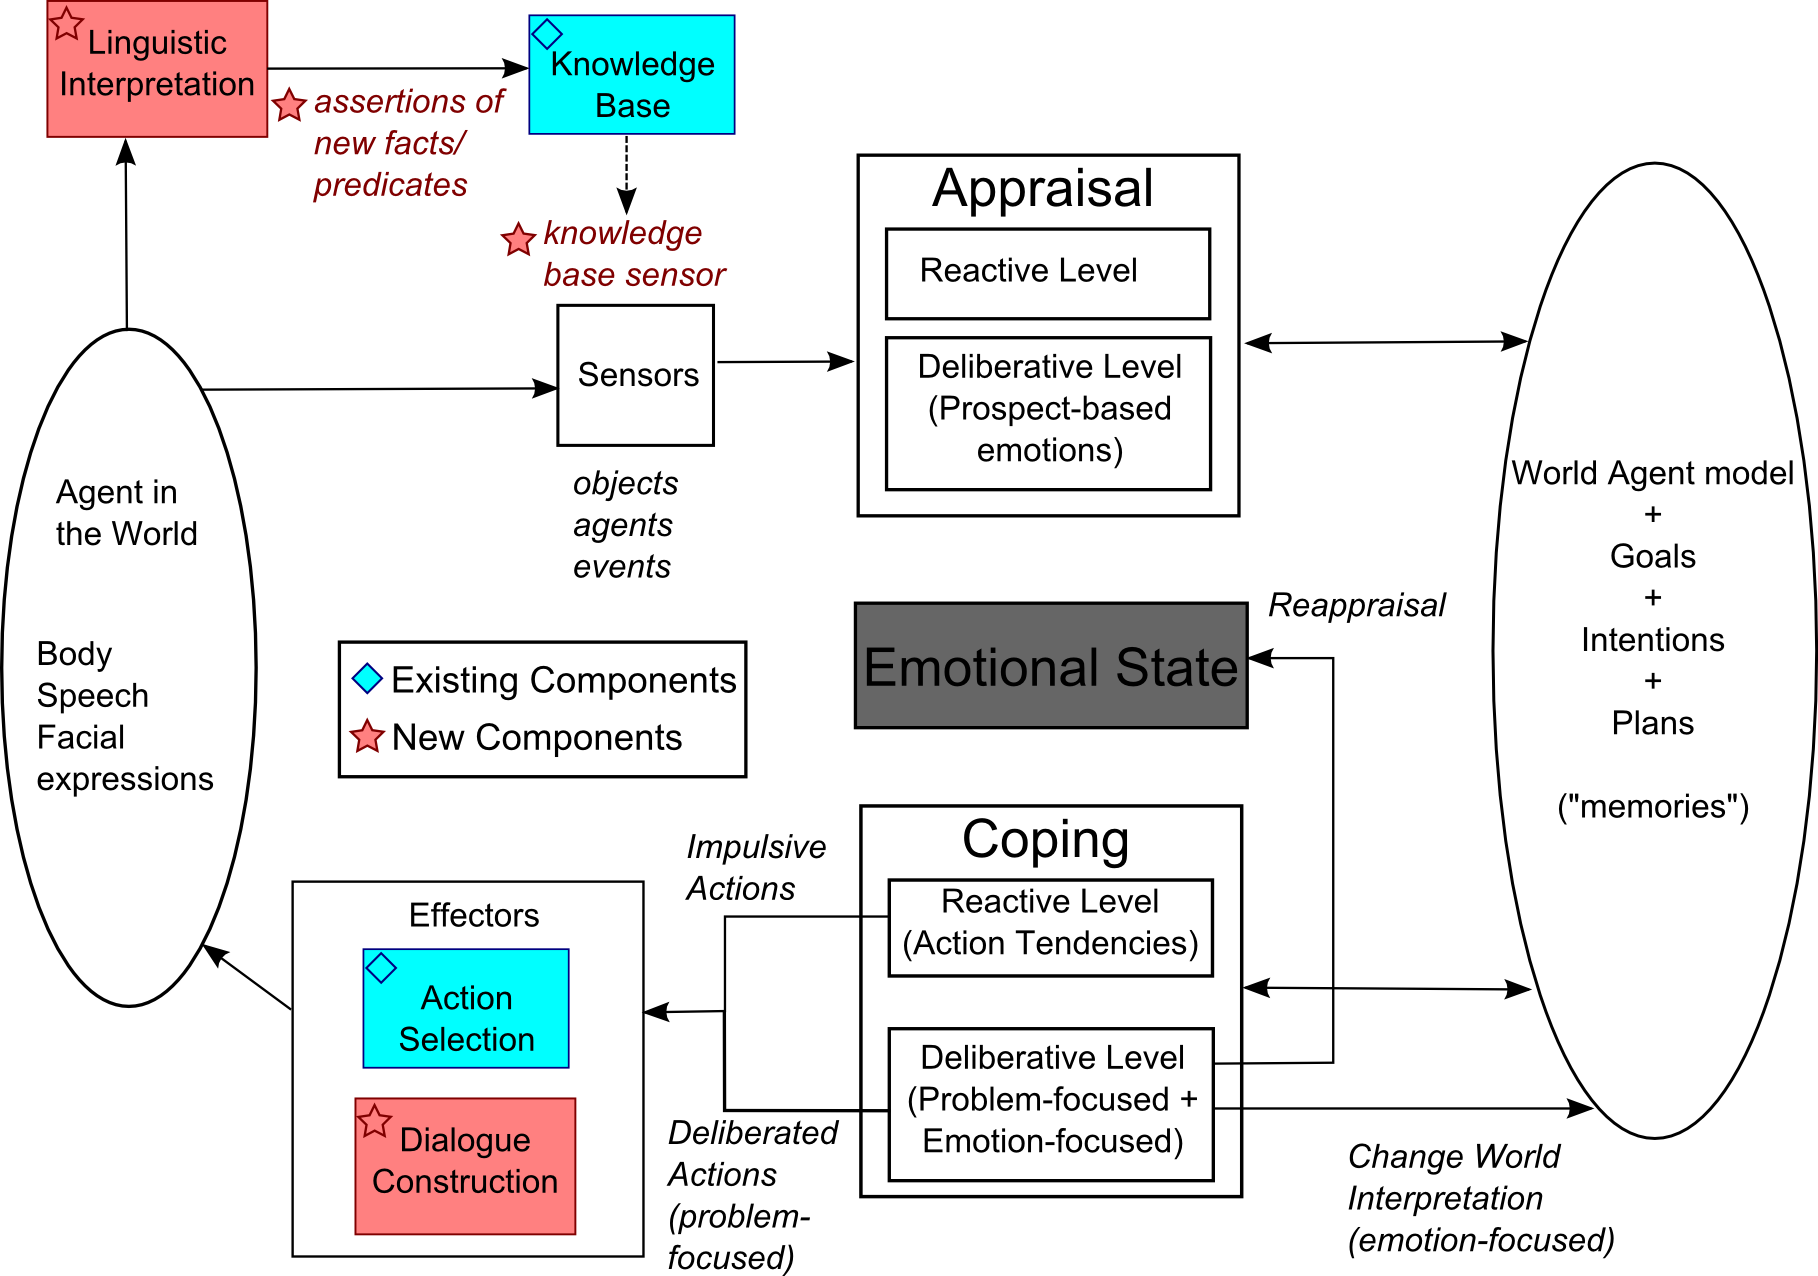
\includegraphics{Graphics/fatimadiagram_modifications_render.png}}
  \caption{An overview of the proposed changes to the FAtiMA architecture.  Objects with diamonds (blue)
  represent existing components that were not displayed in the previous diagram.  Objects with stars (red)
  represent new components.}
  \label{fatima_diagram_modifications}
\end{figure}

FAtiMA's current interaction model is shown in figure ~\ref{fatima_diagram}.
Appraisal and Coping are executed in a cycle.  Actions are appraised, which
affects the emotional state, world state, and memory.  Coping analyzes these
states and affects the world yet again, and these actions are re-appraised.

\subsection{Modifications}

Figure ~\ref{fatima_diagram_modifications} shows the proposed modifications
to the interaction model.  Effectors are split into two categories: Action
Selection and Dialogue Construction.  In addition, a new linguistic interpretation
component is added that causes changes in the state of the knowledge base.

The dialogue construction component will require a search algorithm that is
able to take the current knowledge base state and goal as input, and produce
an optimal assertion that causes the knowledge base to satisfy the goal.

The linguistic interpretation module will be simpler, and will most likely be
implemented with only small modifications to the existing knowledge base system.

\subsubsection{Language Renderer and Derenderer}

Optional components are the language renderer and derenderer.  These, if implemented,
would be able to transform natural language text to logical forms and vice-versa.
This will only be possible if time and other constraints allow, but will most likely
be accomplished through use of OpenCCG\cite{White2011} software.

\section{Conclusion}

This thesis will serve as a proof of concept to demonstrate the potential for dynamically
generated speech among game characters.  Direct generation of dialogue as logical forms
has not yet been attempted to my knowledge, and the implementation of this thesis may
lead to new posisbilities for interaction with intelligent game characters.  Natural language
rendering could also greatly improve believability.  As games grow in complexity, such
technology may become indispensable for the creation of truly dynamic game experiences
while alleviating the burden on game authors.

\section{Timeline}

TODO: I'll discuss this with you.

\bibliographystyle{plain}
\bibliography{references}{}

\end{document}
